\documentclass[aspectratio=169, 10pt]{beamer}

% Theme and Color Scheme
\usetheme{Madrid}
\usecolortheme{whale}

% Custom Colors (Automotive / Tech Palette)
\definecolor{tataBlue}{RGB}{0, 51, 102}
\definecolor{techCyan}{RGB}{0, 128, 128}
\definecolor{accentOrange}{RGB}{204, 85, 0}
\definecolor{bgGray}{RGB}{245, 247, 250}
\definecolor{darkText}{RGB}{30, 30, 30}

\setbeamercolor{palette primary}{bg=tataBlue, fg=white}
\setbeamercolor{palette secondary}{bg=techCyan, fg=white}
\setbeamercolor{palette tertiary}{bg=tataBlue, fg=white}
\setbeamercolor{structure}{fg=tataBlue}
\setbeamercolor{titlelike}{parent=palette primary}
\setbeamercolor{item}{fg=tataBlue}
\setbeamercolor{subitem}{fg=techCyan}
\setbeamercolor{block title}{bg=tataBlue, fg=white}
\setbeamercolor{block body}{bg=bgGray, fg=darkText}
\setbeamercolor{block title example}{bg=techCyan, fg=white}
\setbeamercolor{block body example}{bg=bgGray, fg=darkText}
\setbeamercolor{block title alerted}{bg=accentOrange, fg=white}
\setbeamercolor{block body alerted}{bg=bgGray, fg=darkText}

% Packages
\usepackage{amsmath,amssymb,amsfonts}
\usepackage{booktabs}
\usepackage{tikz}
\usetikzlibrary{arrows.meta, positioning, shapes.geometric}
\usepackage{microtype}

% Remove Navigation Symbols
\setbeamertemplate{navigation symbols}{}

% Custom Footline
\setbeamertemplate{footline}{
  \leavevmode%
  \hbox{%
  \begin{beamercolorbox}[wd=.333333\paperwidth,ht=2.25ex,dp=1ex,center]{author in head/foot}%
    \usebeamerfont{author in head/foot}\insertshortauthor
  \end{beamercolorbox}%
  \begin{beamercolorbox}[wd=.333333\paperwidth,ht=2.25ex,dp=1ex,center]{title in head/foot}%
    \usebeamerfont{title in head/foot}Zeroth Review -- IVN Capstone
  \end{beamercolorbox}%
  \begin{beamercolorbox}[wd=.333333\paperwidth,ht=2.25ex,dp=1ex,right]{date in head/foot}%
    \usebeamerfont{date in head/foot}\insertframenumber{} / \inserttotalframenumber\hspace*{2ex}
  \end{beamercolorbox}}%
  \vskip0pt%
}

% Title Page Information
\title[Root Cause Isolation in Multi-ECU Networks]{Automated Root Cause Isolation in Multi-ECU Networks Using Signal Dependency Mapping and UDS Diagnostics in Vector CANoe}
\subtitle{Capstone Project -- Zeroth Review (Review 0)}
\author[Student Name]{Student Name \\ \small Register No: [Register Number]}
\institute[Tata Tech Capstone]{Department of Electronics and Communication Engineering \\ In-Vehicle Networking (IVN) Capstone | Tata Technologies TechPulse}
\date{\today}

\begin{document}

% Slide 1: Title
\begin{frame}
  \titlepage
\end{frame}

% Slide 2: Problem Statement
\begin{frame}{Problem Statement}
  \begin{itemize}
    \item \textbf{Complex In-Vehicle Architectures:} Modern vehicles integrate 70+ ECUs interconnected across multi-bus networks (CAN / CAN-FD) sharing critical real-time telemetry.
    \item \textbf{Cross-ECU Functional Coupling:} Control algorithms (e.g., ADAS, ESP, TCM, ECM) rely on continuous signal exchanges from shared sensors (e.g., Wheel Speed, Throttle Angle, Yaw Rate).
    \item \textbf{Fault Propagation Cascade:} Failure of a single upstream sensor or transmitter node corrupts or halts broadcasted signals across the bus.
    \item \textbf{Secondary Diagnostic Trouble Code (DTC) Flood:} Downstream recipient ECUs fail to receive valid periodic data and trigger symptom-induced DTCs (e.g., ``U0100 - Lost Communication with ECM'', ``Invalid Data Received'').
    \item \textbf{Diagnostic Ambiguity:} Multiple ECUs log concurrent faults simultaneously, masking the actual root-cause node and defect location.
  \end{itemize}
\end{frame}

% Slide 3: Why It Matters (Real-World Impact)
\begin{frame}{Why It Matters -- Real-World Automotive Impact}
  \begin{itemize}
    \item \textbf{Alarm Flood / Symptom Avalanche:} Diagnostic technicians encounter 5--15 simultaneous DTCs across disparate ECUs originating from one isolated component fault.
    \item \textbf{High ``No Fault Found'' (NFF) Rates:} Secondary ECUs (e.g., Transmission or Body Control) are mistakenly flagged, removed, and replaced despite having no hardware failure.
    \item \textbf{Severe Warranty \& Repair Costs:} OEM warranty claims and service bay diagnostics suffer from prolonged manual troubleshooting.
    \item \textbf{Increased Mean Time to Repair (MTTR):} Service technicians spend hours manually tracing wiring harnesses and decoding individual ECU fault trees.
    \item \textbf{Safety \& Compliance Risks:} Inability to rapidly isolate critical sensor faults impairs functional safety compliance (ISO 26262 ASIL targets) and vehicle uptime.
  \end{itemize}
\end{frame}

% Slide 4: Proposed Solution
\begin{frame}{Proposed Solution}
  \begin{itemize}
    \item \textbf{Automated Diagnostic Correlation Framework:} Implement an intelligent root-cause isolation architecture simulated entirely within \textbf{Vector CANoe}.
    \item \textbf{DBC-Driven Signal Dependency Mapping:}
    \begin{itemize}
      \item Extract transmitter-receiver relationships directly from the CAN database (.DBC).
      \item Construct a Directed Acyclic Dependency Graph (DAG) mapping primary signal producers to dependent subscriber ECUs.
    \end{itemize}
    \item \textbf{UDS Protocol Interrogation (ISO 14229 / ISO 15765-2):}
    \begin{itemize}
      \item Deploy an automated Diagnostic Master node in CANoe using UDS services.
      \item Query active DTC statuses (Service \texttt{0x19}: \textit{ReadDTCInformation}) and freeze-frame sensor snapshots (Service \texttt{0x22}: \textit{ReadDataByIdentifier}).
    \end{itemize}
    \item \textbf{Algorithmic Root Cause Pruning:} Traverse the dependency graph to prune symptomatic secondary DTCs and pinpoint the primary root-cause ECU and fault mode in real time.
  \end{itemize}
\end{frame}

% Slide 5: Project Objectives
\begin{frame}{Project Objectives}
  \begin{block}{Primary Objective}
    \begin{itemize}
      \item \textbf{Develop and simulate an automated diagnostic framework in Vector CANoe} that isolates primary root-cause faults across multi-ECU CAN networks by correlating cross-node signal dependencies with UDS diagnostic trouble codes.
    \end{itemize}
  \end{block}

  \vspace{0.5cm}

  \begin{block}{Secondary Objective}
    \begin{itemize}
      \item \textbf{Design an interactive CANoe test panel and CAPL automation suite} to inject synthetic sensor/bus faults, dynamically visualize fault propagation across nodes, and quantitatively benchmark isolation latency against manual multi-ECU DTC inspection.
    \end{itemize}
  \end{block}
\end{frame}

% Slide 6: Literature Review (Part 1 - Automated Diagnostics & UDS)
\begin{frame}{Literature Review -- UDS Diagnostics \& Test Automation}
  \begin{itemize}
    \item \textbf{Varshney, Joshi, and Namrata (IEEE I2CT, 2019) \cite{varshney2019}:}
    \begin{itemize}
      \item \textit{Focus:} Automated testing of ECU diagnostic lifecycle using Vector VT System and CAPL in Hardware-in-the-Loop (HIL) environments.
      \item \textit{Relevance:} Demonstrated CAPL-driven UDS DTC qualification and fault injection automation for single ECU validation.
    \end{itemize}
    \vspace{0.3cm}
    \item \textbf{Hu, Hou, Guo, and Sun (IEEE CAC, 2019) \cite{hu2019}:}
    \begin{itemize}
      \item \textit{Focus:} Design and implementation of a CAN-based UDS diagnostic system for integrated Body Control Modules (BCM) using Vector CANoe.
      \item \textit{Relevance:} Validated CANoe-based simulation of UDS services (ISO 14229) for automated request-response diagnostic handling.
    \end{itemize}
  \end{itemize}
\end{frame}

% Slide 7: Literature Review (Part 2 - Model-Based Diagnosis & Networks)
\begin{frame}{Literature Review -- Fault Propagation \& Vehicle Networks}
  \begin{itemize}
    \item \textbf{Nyberg (IEEE Trans. Control Syst. Technol., 2002) \cite{nyberg2002}:}
    \begin{itemize}
      \item \textit{Focus:} Model-based diagnosis and structural fault isolation algorithms applied to automotive powertrain systems.
      \item \textit{Relevance:} Formulated analytical isolation techniques to distinguish primary hardware faults from downstream symptoms.
    \end{itemize}
    \vspace{0.3cm}
    \item \textbf{Siegel, Erb, and Sarma (IEEE Trans. Intell. Transp. Syst., 2018) \cite{siegel2018}:}
    \begin{itemize}
      \item \textit{Focus:} Comprehensive survey of connected vehicle architectures, telemetry protocols, and distributed diagnostic paradigms.
      \item \textit{Relevance:} Highlighted the critical challenge of cross-ECU fault propagation in decentralized in-vehicle network architectures.
    \end{itemize}
  \end{itemize}
\end{frame}

% Slide 8: Research Gap
\begin{frame}{Research Gap}
  \begin{itemize}
    \item \textbf{Isolated Single-ECU Focus in Existing Tooling:} Current diagnostic test setups validate UDS DTC handling per ECU in isolation, ignoring network-wide cascading fault propagation.
    \item \textbf{Lack of Semantic DBC Topology Integration:} Machine learning / statistical anomaly detection schemes analyze raw CAN payloads without leveraging the structured publisher-subscriber signal definitions present in OEM .DBC databases.
    \item \textbf{Absence of Real-Time Interactive SIL Implementations:} Theoretical graph/model-based root-cause algorithms remain offline academic formulations rather than executable, deployable workflows inside industry-standard Software-in-the-Loop (SIL) environments like \textbf{Vector CANoe}.
    \item \textbf{Manual Workshop Diagnostic Dependency:} Aftermarket and OEM service tools present flat lists of DTCs, requiring manual technician correlation with zero automated symptom filtering.
  \end{itemize}
\end{frame}

% Slide 9: Project Architecture & Simulated Nodes (1/2)
% Slide 9: Project Architecture & Simulated Nodes
\begin{frame}{Project Details -- Network Architecture \& Simulated Nodes}
  \begin{itemize}
    \item \textbf{Network Specification:} High-Speed CAN Bus (500 kbps) specified via custom database (\texttt{Powertrain\_Body\_Network.dbc}).
    \item \textbf{Simulated ECUs (Vector CANoe Environment):}
    \begin{itemize}
      \item \textbf{Engine Control Module (ECM):} Transmits Engine Speed, Throttle Position, Engine Coolant Temp; logs primary sensor DTCs (e.g., $P0120$).
      \item \textbf{Transmission Control Module (TCM):} Receives ECM torque/RPM and ABS wheel speed for shift decisions; logs secondary data-invalid DTCs (e.g., $U0401$).
      \item \textbf{Anti-Lock Braking System (ABS / ESP):} Transmits 4-wheel speeds, yaw rate, brake pressure; logs wheel speed sensor fault ($C0035$).
      \item \textbf{Body Control Module (BCM):} Transmits vehicle state, cluster indicators, door/lighting telemetry.
      \item \textbf{Diagnostic Master Node (Tester):} Automated UDS client (ISO 15765-2 / ISO 14229) initiating diagnostic sessions and running isolation algorithms.
    \end{itemize}
  \end{itemize}
\end{frame}

% Slide 10: End-to-End System Workflow Diagram
\begin{frame}{Methodology -- End-to-End System Workflow Diagram}
  \begin{itemize}
    \item \textbf{System Pipeline: From Fault Occurrence to Automated Root Cause Isolation:}
  \end{itemize}
  \vspace{0.2cm}
  \centering
  \resizebox{0.92\textwidth}{!}{
    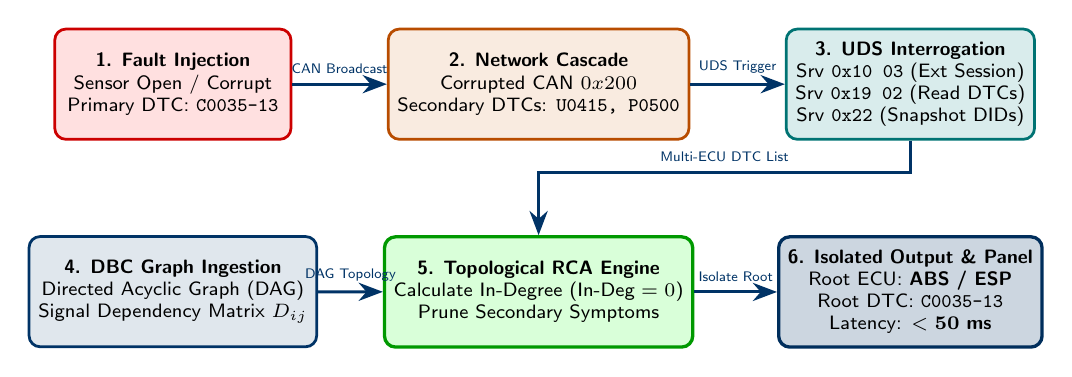
\begin{tikzpicture}[
      node distance=1.2cm and 1.2cm,
      every node/.style={font=\sffamily\scriptsize},
      fault/.style={rectangle, draw=red!80!black, fill=red!12, rounded corners=4pt, line width=1pt, align=center, minimum height=1.4cm, minimum width=3.0cm},
      symptom/.style={rectangle, draw=accentOrange!90!black, fill=accentOrange!12, rounded corners=4pt, line width=1pt, align=center, minimum height=1.4cm, minimum width=3.0cm},
      diag/.style={rectangle, draw=techCyan!90!black, fill=techCyan!15, rounded corners=4pt, line width=1pt, align=center, minimum height=1.4cm, minimum width=3.0cm},
      block/.style={rectangle, draw=tataBlue, fill=tataBlue!12, rounded corners=4pt, line width=1pt, align=center, minimum height=1.4cm, minimum width=3.0cm},
      rca/.style={rectangle, draw=green!60!black, fill=green!15, rounded corners=4pt, line width=1.2pt, align=center, minimum height=1.4cm, minimum width=3.2cm},
      outputb/.style={rectangle, draw=tataBlue!90!black, fill=tataBlue!20, rounded corners=4pt, line width=1.2pt, align=center, minimum height=1.4cm, minimum width=3.0cm},
      arrow/.style={-{Stealth[scale=1.1]}, line width=1.1pt, color=tataBlue},
      carrow/.style={-{Stealth[scale=1.1]}, line width=1.1pt, color=accentOrange}
    ]
      % Top Row: Fault to Diagnostic Interrogation
      \node[fault] (step1) {\textbf{1. Fault Injection}\\\scriptsize Sensor Open / Corrupt\\\scriptsize Primary DTC: \texttt{C0035-13}};
      \node[symptom, right=of step1] (step2) {\textbf{2. Network Cascade}\\\scriptsize Corrupted CAN $0x200$\\\scriptsize Secondary DTCs: \texttt{U0415, P0500}};
      \node[diag, right=of step2] (step3) {\textbf{3. UDS Interrogation}\\\scriptsize Srv \texttt{0x10 03} (Ext Session)\\\scriptsize Srv \texttt{0x19 02} (Read DTCs)\\\scriptsize Srv \texttt{0x22} (Snapshot DIDs)};

      % Bottom Row: Graph Ingestion to Isolation & Report
      \node[block, below=1.2cm of step1] (step4) {\textbf{4. DBC Graph Ingestion}\\\scriptsize Directed Acyclic Graph (DAG)\\\scriptsize Signal Dependency Matrix $D_{ij}$};
      \node[rca, below=1.2cm of step2] (step5) {\textbf{5. Topological RCA Engine}\\\scriptsize Calculate In-Degree ($\text{In-Deg}=0$)\\\scriptsize Prune Secondary Symptoms};
      \node[outputb, below=1.2cm of step3] (step6) {\textbf{6. Isolated Output \& Panel}\\\scriptsize Root ECU: \textbf{ABS / ESP}\\\scriptsize Root DTC: \textbf{\texttt{C0035-13}}\\\scriptsize Latency: $\mathbf{<50\text{ \textbf{ms}}}$};

      % Connecting Arrows
      \draw[arrow] (step1) -- node[above, font=\sffamily\tiny]{CAN Broadcast} (step2);
      \draw[arrow] (step2) -- node[above, font=\sffamily\tiny]{UDS Trigger} (step3);
      \draw[arrow] (step3.south) -- ++(0,-0.4) -| (step5.north) node[pos=0.25, above, font=\sffamily\tiny]{Multi-ECU DTC List};
      \draw[arrow] (step4) -- node[above, font=\sffamily\tiny]{DAG Topology} (step5);
      \draw[arrow] (step5) -- node[above, font=\sffamily\tiny]{Isolate Root} (step6);
    \end{tikzpicture}
  }
\end{frame}

% Slide 11: Methodology - Dependency Modeling & Fault Mapping
\begin{frame}{Methodology -- Signal Dependency Modeling \& Graph Formulation}
  \begin{itemize}
    \item \textbf{CAN Database Parsing (.DBC Ingestion):}
    \begin{itemize}
      \item Automated extraction of message IDs, signal bit positions, cycle times (10ms--100ms), and transmitter-receiver bindings.
    \end{itemize}
    \item \textbf{Directed Acyclic Dependency Graph (DAG) Construction:}
    \begin{itemize}
      \item \textit{Vertices ($V$):} Physical sensors, published CAN signals, and software ECU modules.
      \item \textit{Directed Edges ($E$):} Signal flow direction $Node_{TX} \xrightarrow{Signal_k} Node_{RX}$ defining functional dependencies.
      \item \textit{Dependency Matrix ($D_{ij}$):} Encodes binary/weighted dependencies where $D_{ij} = 1$ indicates $ECU_j$ depends on $ECU_i$.
    \end{itemize}
    \item \textbf{Cross-ECU Fault Propagation Mapping:}
    \begin{itemize}
      \item Pre-defines causal symptom chains (e.g., Wheel Speed Sensor failure $\rightarrow$ ABS fault $C0035$ $\rightarrow$ TCM invalid data $U0415$ $\rightarrow$ ECM limp mode $P0500$).
    \end{itemize}
  \end{itemize}
\end{frame}

% Slide 12: Implementation - CANoe Simulation & Fault Injection
\begin{frame}{Implementation -- Vector CANoe Simulation \& Fault Injection Pipeline}
  \begin{itemize}
    \item \textbf{Multi-Node CAPL Simulation Environment:}
    \begin{itemize}
      \item Independent CAPL scripts assigned to each network node simulating cyclic broadcast and internal control loops.
      \item Embedded diagnostic server stack on each ECU handling ISO 14229 UDS requests.
    \end{itemize}
    \item \textbf{CAPL Fault Injection Engine:}
    \begin{itemize}
      \item \textit{Sensor Level:} Signal corruption, out-of-range injection, stuck-at-constant, and signal noise.
      \item \textit{Protocol Level:} Alive counter freezing, CRC checksum mismatch, and intermittent frame dropouts.
      \item \textit{Bus Level:} Complete node communication timeout and bus-off triggering.
    \end{itemize}
    \item \textbf{On-Node Fault Debounce \& DTC Setting:}
    \begin{itemize}
      \item ECUs qualify faults using internal timers (200ms debounce) and update standard DTC status bytes (`TestFailed`, `ConfirmedDTC`).
    \end{itemize}
  \end{itemize}
\end{frame}

% Slide 13: Implementation - UDS Interrogation & Root Cause Isolation
\begin{frame}{Implementation -- UDS Diagnostic Interrogation \& Isolation Algorithm}
  \begin{itemize}
    \item \textbf{Automated Diagnostic Master Workflow (CAPL):}
    \begin{itemize}
      \item \textit{Session Control:} Broadcasts UDS Service \texttt{0x10 03} (\textit{Extended Diagnostic Session}).
      \item \textit{DTC Extraction:} Queries Service \texttt{0x19 02} (\textit{ReadDTCByStatusMask} with mask \texttt{0x09}) across all ECUs over ISO-TP (ISO 15765-2).
      \item \textit{Freeze-Frame Snapshot:} Issues Service \texttt{0x22} (\textit{ReadDataByIdentifier}) to fetch sensor parameters at the moment of failure.
    \end{itemize}
    \item \textbf{Topological Root Cause Pruning Algorithm:}
    \begin{itemize}
      \item Ingests aggregated multi-ECU active DTC list into the pre-compiled Dependency DAG.
      \item Traverses graph upstream to identify root-level vertices having in-degree zero among active faults.
      \item Suppresses downstream symptomatic DTCs (e.g., flags $U0415$ on TCM as secondary symptom of $C0035$ on ABS).
      \item Outputs primary root-cause ECU, failed component/sensor ID, and confidence metric in real time.
    \end{itemize}
  \end{itemize}
\end{frame}

% Slide 14: Implementation - UI Dashboard & Verification Workflow
\begin{frame}{Implementation -- Interactive Panel Dashboard \& Verification Workflow}
  \begin{itemize}
    \item \textbf{Vector CANoe Interactive Panel Interface:}
    \begin{itemize}
      \item Live telemetry display (Engine Speed, Vehicle Speed, Gear Status, Wheel Speeds).
      \item Fault Injection Control Panel (drop-down selection for fault type, target node, and injection trigger).
      \item Root Cause Diagnostic Dashboard: Real-time active DTC table, causal path visualization, and isolated root cause report.
    \end{itemize}
    \item \textbf{Verification \& Performance Benchmarking:}
    \begin{itemize}
      \item Diagnostic trace logging in Vector BLF and ASC formats for post-test analysis.
      \item Quantitative benchmarking: Automated root cause isolation latency ($<500\text{ ms}$) vs. manual diagnostic tree navigation ($>15\text{ mins}$).
      \item Verification against $100\%$ synthetic fault test matrices (sensor faults, bus faults, cascading multi-node failures).
    \end{itemize}
  \end{itemize}
\end{frame}

% Slide 15: Alignment with Tata Technologies Assessment Rubric
\begin{frame}{Alignment with Assessment Plan \& Deliverables}
  \begin{itemize}
    \item \textbf{DBC File Creation (20 Marks):} Comprehensive network DBC defining 5 nodes, 15+ messages, 40+ signals, scaling, offsets, and attributes.
    \item \textbf{Panel Design (20 Marks):} Interactive Vector CANoe UI for manual/automated fault injection, real-time node state telemetry, and diagnostic output display.
    \item \textbf{CAPL Scripting (20 Marks):} Optimized, modular CAPL code implementing node behavior, UDS server stacks (ISO 14229), and diagnostic client scripts.
    \item \textbf{Integration \& Simulation (20 Marks):} Seamless co-simulation of nodes, panels, and scripts with validated execution and BLF/ASC trace logs.
    \item \textbf{Documentation \& Innovation (20 Marks):} Comprehensive technical report, architecture flowcharts, 5--10 min video demonstration, and novel cross-ECU root cause logic.
  \end{itemize}
\end{frame}

% Slide 16: References (IEEE Format)
\begin{frame}{References (IEEE Format)}
  \begin{thebibliography}{99}
    \bibitem{varshney2019}
    A.~Varshney, S.~D.~Joshi, and K.~Namrata, ``Automated Testing of Faults of an Automotive System,'' in \emph{Proc. 2019 IEEE 5th Int. Conf. for Convergence in Technology (I2CT)}, Bombay, India, 2019, pp.~1--4, doi: 10.1109/I2CT45611.2019.9033751.

    \bibitem{hu2019}
    D.~Hu, D.~Hou, K.~Guo, and C.~Sun, ``Design and Implementation of Diagnostic System for Integrated Body Controller Based on CAN Bus,'' in \emph{Proc. 2019 Chinese Automation Congress (CAC)}, Hangzhou, China, 2019, pp.~4453--4457, doi: 10.1109/CAC48633.2019.8996582.

    \bibitem{nyberg2002}
    M.~Nyberg, ``Model-Based Diagnosis of an Automotive Powertrain with Real-Time Application,'' \emph{IEEE Trans. Control Syst. Technol.}, vol.~10, no.~6, pp.~879--888, Nov. 2002, doi: 10.1109/TCST.2002.804121.

    \bibitem{siegel2018}
    J.~E.~Siegel, D.~C.~Erb, and S.~E.~Sarma, ``A Survey of the Connected Vehicle Landscape---Architectures, Enabling Technologies, Applications, and Solutions,'' \emph{IEEE Trans. Intell. Transp. Syst.}, vol.~19, no.~3, pp.~1032--1049, Mar. 2018, doi: 10.1109/TITS.2017.2749459.

    \bibitem{iso14229}
    \emph{Road vehicles --- Unified diagnostic services (UDS) --- Part 1: Application layer}, ISO Standard 14229-1:2020, International Organization for Standardization, Geneva, Switzerland, 2020.
  \end{thebibliography}
\end{frame}

\end{document}
